% Paper 2: Mechanism decomposition of Atlantic F_ovS
% Target journal: Communications Earth & Environment
%
% The recommended length is less than ~5,000 words.


\documentclass[11pt,a4paper]{article}


\usepackage[utf8]{inputenc}
\usepackage[T1]{fontenc}
\usepackage[margin=2.5cm]{geometry}
\usepackage{graphicx}
\usepackage{amsmath,amssymb}
\usepackage{hyperref}
\hypersetup{colorlinks=true, linkcolor=black, citecolor=black, urlcolor=black}
\usepackage[numbers,sort&compress]{natbib}
\usepackage{lineno}
\usepackage[font=small,labelfont=bf]{caption}
\usepackage{subcaption}
\usepackage{booktabs}
\usepackage{authblk}

% =====================================================================
% Figure layout toggle
% ---------------------------------------------------------------------
% \splitfigsfalse  -> use the single combined PDF per figure
%                     (FigureN.pdf). RECOMMENDED for journal submission.
% \splitfigsfalse   -> include each panel as a separate PDF
%                     (FigureNa.pdf, FigureNb.pdf, ...) glued together
%                     with subcaption. RECOMMENDED for editing — you
%                     can swap a single panel without re-rendering the
%                     others, and reviewers' panel-specific comments
%                     map cleanly to file names.
% =====================================================================
\newif\ifsplitfigs
\splitfigsfalse

\newcommand{\Fovs}{F_\mathrm{ovS}}
\newcommand{\dFv}{\Delta F_v}
\newcommand{\dFs}{\Delta F_s}
\newcommand{\dFc}{\Delta F_\mathrm{cross}}

\title{\textbf{\Large The Atlantic is freshening for opposing reasons --- and only one points toward AMOC collapse
}}

\author[2,3,1]{Masoud Rostami\footnote{Corresponding authors: Masoud Rostami (\texttt{mrostami@lmd.ens.fr}) and Li-Yun Fu (\texttt{lfu@upc.edu.cn})}}
\author[1]{Bijan Fallah}
\author[4]{Junxin Guo}
\author[2,5]{Li-Yun Fu}

\affil[1]{\small Potsdam Institute for Climate Impact Research (PIK), Member of the Leibniz Association, P.O. Box 6012 03, D-14412 Potsdam, Germany}
\affil[2]{School of Geosciences, China University of Petroleum (East China), Qingdao, China}
\affil[3]{Laboratoire de M\'{e}t\'{e}orologie Dynamique (LMD) / IPSL, ENS-PSL Universit\'{e}, Ecole Polytechnique-Institut Polytechnique de Paris, Sorbonne Universit\'{e}, CNRS, Paris, France}
\affil[4]{MSU-BIT-SMBU Joint Research Center of Applied Mathematics, Shenzhen MSU-BIT University, Shenzhen, China}
\affil[5]{Qingdao National Laboratory for Marine Science and Technology, Qingdao, China}

\date{} % optional

\graphicspath{{./figures/}}




\begin{document}
\maketitle

\begin{abstract}
Climate models consistently project a weakening of the Atlantic meridional overturning circulation (AMOC) under continued warming, but the short observational record forces scientists to rely on ocean reanalyses – and these reanalyses do not agree on why the Atlantic is freshening. Four widely used reanalyses all confirm that the Atlantic is in a bistable (tipping‑prone) regime, yet they split into two opposing camps when asked what drives the recent freshening. One group points to changes in ocean currents (a velocity‑driven process), the other to a redistribution of salt (the direct signature of an active AMOC feedback). Strikingly, climate models exhibit the same mechanistic split. When future AMOC projections are grouped by mechanism, the two camps yield systematically different weakening rates: models that follow the salt‑redistribution story project a much stronger decline than those that follow the current‑driven story. This hidden mechanism‑dependent uncertainty – amounting to a large gap in projected AMOC weakening – is not captured by current observational constraints, which implicitly average over the two interpretations. Our results show that trusting any single projection requires first understanding which mechanism is actually at work, and that targeted observations of Atlantic salinity are urgently needed to resolve this ambiguity.
\end{abstract}

\linenumbers


The Atlantic Meridional Overturning Circulation (AMOC) continuously transports heat and salt northward, playing a critical role in global climate \citep{Weijer2019, BuckleyMarshall2016, IPCC_AR6_Chapter9}. Physically, the surface return flow scales up the Florida Current and the Gulf Stream, carrying buoyancy poleward before extensive heat loss in the subpolar North Atlantic triggers deep convection and the formation of North Atlantic Deep Water (NADW). While Eulerian-mean observations characterize this overturning as a zonally-averaged streamfunction, the actual mass transport relies on complex, eddying Lagrangian pathways that navigate the geographic and thermal constraints of the subpolar gyre. A sustained weakening of this circulation poses severe ecological and societal risks \citep{Rahmstorf1996, vanWesten2024, ManabeStouffer1988}. Reconstructions suggest the AMOC has declined by $\sim$15\% since the mid-twentieth century \citep{Caesar2018, Caesar2021, RahmstorfCaesar2026}, and statistical early-warning signals raise concerns about future stability \citep{Boers2021, Ditlevsen2023}. However, following IPCC AR6 assessments, there remains low confidence in an abrupt, 21st-century AMOC collapse \citep{IPCC_AR6_Chapter9}. Nevertheless, the potential for a tipping point remains a profound low-probability, high-impact risk. Because direct continuous measurements span only two decades at 26.5\textdegree N (RAPID) \citep{McCarthy2015, Smeed2018, Bryden2005} and one decade in the subpolar region (OSNAP) \citep{Lozier2019, FrajkaWilliams2019}, establishing physical constraints on future changes relies heavily on model projections and ocean reanalyses \citep{Karspeck2017, Jackson2019}. All such projections are inherently model-dependent. Different models, different reanalyses, and different data assimilation techniques can yield divergent -- sometimes contradictory -- answers, raising a fundamental question: how much confidence can we place in any single projection?

A critical metric for assessing this tipping-point risk is the overturning freshwater transport at 34.5°S, denoted \(F_{\mathrm{ovS}}\). This metric quantifies the net export of freshwater from the Atlantic basin by the overturning circulation and is defined as the depth integral of the product of the overturning velocity (the zonally-averaged meridional velocity after removing the barotropic component) and the salinity anomaly relative to a reference salinity \(S_0 = 35\) PSU (Practical Salinity Unit) \citep{deVriesWeber2005, HofmannRahmstorf2009}. A negative \(F_{\mathrm{ovS}}\) indicates that the AMOC exports freshwater. Consequently, if the overturning slows, freshwater export decreases, driving a net accumulation of salt in the North Atlantic. This basin-scale salinification acts to densify the upper water column and restabilize the sinking branch—the fundamental positive feedback mechanism first proposed by Stommel \citep{Stommel1961}. When this salt-advection feedback operates, the system resides in a \emph{bistable} regime, capable of transitioning between an active overturning state and a sluggish, convection-suppressed state \citep{Rahmstorf1996, Dijkstra2007, vanWesten2024, Cimatoribus2014}. A positive \(F_{\mathrm{ovS}}\), conversely, implies a single stable (monostable) regime. Thus, the sign of \(F_{\mathrm{ovS}}\) dictates whether the Atlantic harbors the physical prerequisites for an AMOC tipping point.

Analyses of observational data and ocean reanalyses show a negative mean \(F_{\mathrm{ovS}}\), placing the present-day Atlantic firmly within the bistable regime \citep{ArumiPlanas2024, Portmann2026}. Yet, recent observed declines in \(F_{\mathrm{ovS}}\) introduce a critical physical ambiguity: the trend could emerge from two fundamentally different mechanisms. Wind-driven alterations in the boundary current system ("velocity-driven" changes) can reduce freshwater transport without invoking profound regime shifts, as these dynamics are largely reversible \citep{Chemke2021}. Conversely, the decline could trace directly to a basin-scale buoyancy perturbation ("salinity-driven" changes) characteristic of an active salt-advection feedback, signaling that the ocean is actively approaching a tipping point \citep{deVriesWeber2005, Drijfhout2011, vanWesten2024, Liu2017, Sgubin2017}. Because current observational constraints focus strictly on the magnitude of the \(F_{\mathrm{ovS}}\) decline, they obscure which physical mechanism is operating. This gap compromises our ability to determine if the freshening signals a future tipping point or merely a temporary fluctuation, directly undermining trust in model-based AMOC projections.

To isolate these processes, we apply an exact diagnostic decomposition that splits the recent change in \(F_{\mathrm{ovS}}\) into a velocity-driven component (\(\Delta F_v\)), a salinity-driven component (\(\Delta F_s\)), and their cross term (\(\Delta F_{\mathrm{cross}}\)). We evaluate this decomposition across four independent, widely used ocean reanalyses (ORAS5 \citep{Zuo2019}, GLORYS12V1 \citep{Lellouche2021}, SODA 3.15.2 \citep{Carton2018}, and ECCO-V4r4 \citep{Forget2015}), spanning the major data-assimilation paradigms and matching the canonical ensemble used in recent emergent-constraint studies \citep{Portmann2026}. We pair this analysis with 15 CMIP6 models. The full per-analysis bookkeeping is detailed in the Supplementary Information, along with the decomposition methodology and statistical tests. Here we show that two leading reanalyses explain the observed Atlantic freshening via entirely opposite mechanisms, carrying profound implications for future AMOC trajectories. This hidden, qualitative uncertainty bypasses existing emergent constraints and directly manifests as a \(\sim\)10-percentage-point divergence in projected AMOC weakening by 2100.

\section*{Results}
\label{sec:Results}
% =========================================================================
% Figure 1: Reanalysis mean state and the mechanism disagreement
% =========================================================================
\begin{figure}
\centering
\ifsplitfigs
  \begin{subfigure}{\linewidth}\centering
    
\includegraphics[width=\linewidth]{Figure1a.pdf}
    \caption{}\label{fig:f1a}
  \end{subfigure}\\[4pt]
  \begin{subfigure}{0.49\linewidth}\centering
    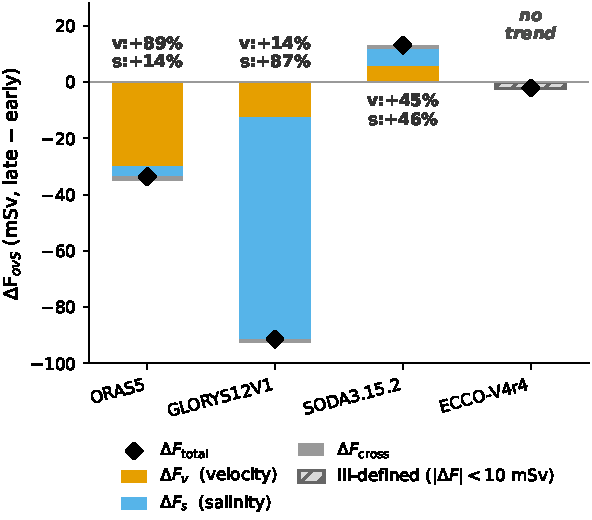
\includegraphics[width=\linewidth]{Figure1b.pdf}
    \caption{}\label{fig:f1b}
  \end{subfigure}\hfill
  \begin{subfigure}{0.49\linewidth}\centering
    
\includegraphics[width=\linewidth]{Figure1c.pdf}
    \caption{}\label{fig:f1c}
  \end{subfigure}
\else
  
\includegraphics[width=\linewidth]{Figure1.pdf}
\fi
\caption{\textbf{Atlantic bistability and opposing mechanisms for freshening.}
\textbf{(a)} Long-term \(F_{\mathrm{ovS}}\) time series at 34.5°S. The shaded region (\(F_{\mathrm{ovS}}<0\)) indicates the bistable regime of the salt-advection feedback, where a weakening AMOC would increase North Atlantic salinity -- a positive feedback that can lead to a collapsed overturning state. Diamonds denote direct hydrography estimates. All four reanalyses have negative mean values, confirming that the Atlantic resides in the bistable regime.
\textbf{(b)} Mechanism decomposition of the \(F_{\mathrm{ovS}}\) change between 1993-2005 and 2013-2025. The change \(\Delta F_{\mathrm{ovS}}\) is split into a velocity-driven part \(\Delta F_v\) (due to circulation changes only), a salinity-driven part \(\Delta F_s\) (due to salinity redistribution only), and a cross term \(\Delta F_{\mathrm{cross}}\) (correlations). ORAS5 is 89\% velocity-driven (circulation change dominates), whereas GLORYS12V1 is 87\% salinity-driven -- the direct fingerprint of active salt-advection feedback. ECCO-V4r4 has \(|\Delta F_{\mathrm{ovS}}|<10\) mSv (mechanism ill-defined, hatched bar).
\textbf{(c)} Vertical profiles of the integrands, revealing that the opposite attributions originate from depth-dependent differences in velocity and salinity anomalies. These opposing mechanisms imply fundamentally different future AMOC trajectories, as quantified in Figure~\ref{fig:cmip6_projection}.}
\label{fig:reanalysis_mechanism}
\end{figure}

\paragraph*{Reanalyses disagree on the mechanism driving AMOC-relevant freshening}

To resolve ambiguity, we apply an exact decomposition that separates the change in \(F_{\mathrm{ovS}}\) into a velocity-driven part (\(\Delta F_v\)), a salinity-driven part (\(\Delta F_s\)), and a cross term (\(\Delta F_{\mathrm{cross}}\)). \(\Delta F_v\) isolates changes that would occur if only the circulation structure changed while salinity remained fixed. \(\Delta F_s\) isolates changes that would occur if only the salinity distribution changed while circulation remained fixed. The cross term accounts for correlations between velocity and salinity anomalies. Applying this decomposition to four independent ocean reanalyses (ORAS5 \citep{Zuo2019}, GLORYS12V1 \citep{Lellouche2021}, SODA 3.15.2 \citep{Carton2018}, ECCO-V4r4 \citep{Forget2015}) yields a previously undocumented finding.

Figure~\ref{fig:reanalysis_mechanism} presents this result. Panel~(a) confirms that all four reanalyses have negative long-term means (from \(-0.009\) to \(-0.116\) Sv), placing the Atlantic in the bistable regime -- consistent with prior knowledge. Trends, however, differ: ORAS5 and GLORYS12V1 show significant declines (\(-1.4\) and \(-4.4\) mSv yr\(^{-1}\), respectively), whereas SODA and ECCO exhibit nearly flat trends. This already suggests a deeper inconsistency.
Panel~(b) resolves that inconsistency. It reveals that ORAS5 attributes 89\% of its decline to \(\Delta F_v\) (velocity-driven), whereas GLORYS12V1 attributes 87\% to \(\Delta F_s\) (salinity-driven) -- the direct fingerprint of active salt-advection feedback. Thus, the two most widely used reanalyses point to opposite physical mechanisms for the same observed freshening. The vertical profiles in panel~(c) show that these opposite attributions originate from depth-dependent differences in velocity and salinity anomalies.

This result fundamentally improves our understanding of Atlantic freshening. The mechanism itself -- not just the magnitude of the \(F_{\mathrm{ovS}}\) decline -- is reanalysis-dependent. Prior knowledge assumed that different reanalyses would agree on the mechanism because they assimilate similar observations. We show they do not. Consequently, any observational constraint that uses reanalysis data to project future AMOC weakening implicitly inherits an invalidated mechanistic assumption. This ambiguity translates directly into substantial uncertainty in near-term AMOC projections, as we demonstrate next using CMIP6 models that naturally split into the same two mechanism classes.

\paragraph*{CMIP6 models mirror the reanalysis split and reveal a 10\% difference in AMOC projections}

The same exact decomposition applied to 12 CMIP6 models that exhibit forced AMOC weakening under SSP5-8.5 (historical 1950--1980 versus 2080--2100) reproduces the mechanistic diversity seen in the reanalyses. As shown in Figure~\ref{fig:cmip6_projection}\textbf{(a)}, six models are salinity-dominant (velocity share \(<40\%\)), five models are velocity-dominant (velocity share \(>60\%\)), and one model is mixed. The two reanalysis end-members -- ORAS5 (velocity-dominant) and GLORYS12V1 (salinity-dominant) -- fall at opposite corners of the CMIP6 cloud. A null test based on 2600 random 30-year segments from piControl runs confirms that these forced signals lie well above internal variability.

The consequence of this mechanistic split for future AMOC weakening is quantified in Figure~\ref{fig:cmip6_projection}\textbf{(b,c)}. When the models are partitioned by mechanism class, the salinity-dominant subset (\(n=6\)) projects a median AMOC weakening of 52\% by 2100 (IQR 47--54\%). In contrast, the velocity-dominant subset (\(n=5\)) projects only 42\% (IQR 32--43\%). The salinity-dominant median is statistically indistinguishable from the observational constraint of \citet{Portmann2026} (51\(\pm\)8\%), whereas the velocity-dominant median is nearly 10 percentage points lower. The continuous Spearman correlation between velocity-share and projected weakening across the same 12 models is consistent in sign ($\rho = -0.46$, $p = 0.14$; Supplementary Fig.~S6), directionally supporting the binary partition but not yet significant at the 5\% level given the small ensemble size; we therefore report the 10-percentage-point gap as a tentative upper bound on the mechanism-conditioned uncertainty rather than a definitive measurement, and treat the bistable-only subset (Figure~\ref{fig:bistable_subset}, $n=4$) as the cleanest like-with-like comparison to the four observational reanalyses, all of which sit in the bistable regime. The persistence of the gap in that subset rules out the well-known CMIP6 fresh bias in the South Atlantic as a confounding factor.

The mechanism split is not an artefact of model resolution. Within our ensemble, the two MPI-ESM1-2 siblings share identical physics but differ in ocean resolution (LR: $\sim$1.5\textdegree, HR: $\sim$0.4\textdegree). After applying the barotropic correction, both are classified as velocity-dominant, ruling out resolution as the sole discriminator. The same barotropic correction has long been recognised as essential in idealised water-hosing intercomparisons \citep{Stouffer2006}, where mass-budget closure across the diagnostic section determines whether the simulated freshwater fingerprint is interpretable as an overturning signal.

% =========================================================================
% Figure 2: CMIP6 validation and the 10-percentage-point projection gap
% =========================================================================
\begin{figure}
\centering
\ifsplitfigs
  \begin{subfigure}{0.33\linewidth}\centering
    
\includegraphics[width=\linewidth]{Figure2a.pdf}
    \caption{}\label{fig:f2a}
  \end{subfigure}\hfill
  \begin{subfigure}{0.33\linewidth}\centering
    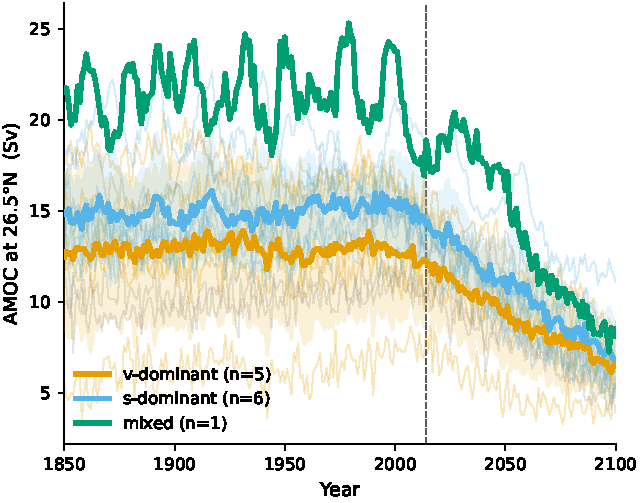
\includegraphics[width=\linewidth]{Figure2b.pdf}
    \caption{}\label{fig:f2b}
  \end{subfigure}\hfill
  \begin{subfigure}{0.32\linewidth}\centering
    
\includegraphics[width=\linewidth]{Figure2c.pdf}
    \caption{}\label{fig:f2c}
  \end{subfigure}
\else
  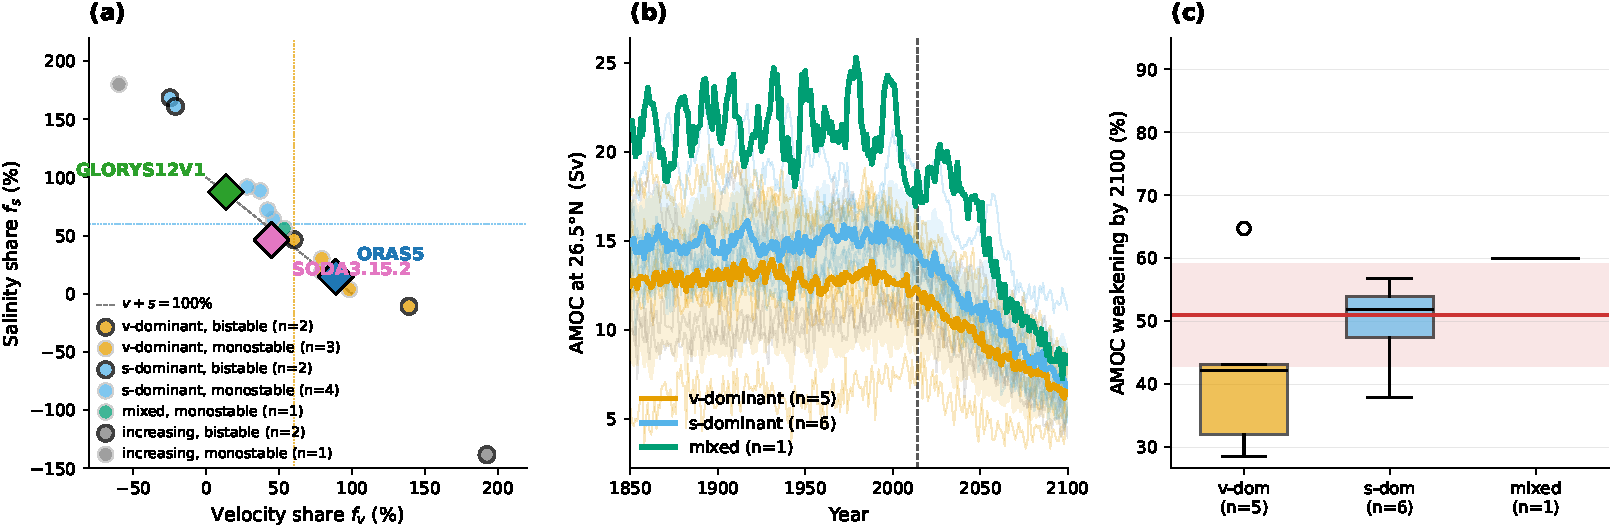
\includegraphics[width=\linewidth]{Figure2.pdf}
\fi
\caption{\textbf{CMIP6 mirrors the reanalysis split and reveals a hidden 10\% uncertainty in AMOC weakening.}
\textbf{(a)} Velocity-share vs salinity-share for 12 CMIP6 models with forced AMOC weakening. Symbol edge: black = bistable baseline, grey = monostable. Reanalysis products are plotted as diamonds (ORAS5 in dark blue, GLORYS12V1 in dark green) and lie at opposite corners of the CMIP6 cloud. CMIP6 model identities are documented in the Supplementary Information; only the four reanalyses are labelled here for clarity.
\textbf{(b)} Mechanism-conditional historical and future AMOC at $26.5^\circ\mathrm{N}$ for CMIP6 models, grouped by mechanism: salinity-dominant (light blue), velocity-dominant (orange) and mixed (green). Vertical dashed line marks the historical $\rightarrow$ SSP5-8.5 transition (2014).
\textbf{(c)} Projected weakening by 2100: salinity-dominant median 52\%, velocity-dominant median 42\% -- a $\sim10$-point gap. Red horizontal line and shaded band: observational constraint from \citet{Portmann2026} ($51\pm8\%$).}
\label{fig:cmip6_projection}
\end{figure}

% =========================================================================
% Figure 3: AMOC projections for bistable-only subset
% =========================================================================
\begin{figure}
\centering
\ifsplitfigs
  \begin{subfigure}{0.49\linewidth}\centering
    
\includegraphics[width=\linewidth]{Figure3a.pdf}
    \caption{}\label{fig:f3a}
  \end{subfigure}\hfill
  \begin{subfigure}{0.49\linewidth}\centering
    
\includegraphics[width=\linewidth]{Figure3b.pdf}
    \caption{}\label{fig:f3b}
  \end{subfigure}
\else
  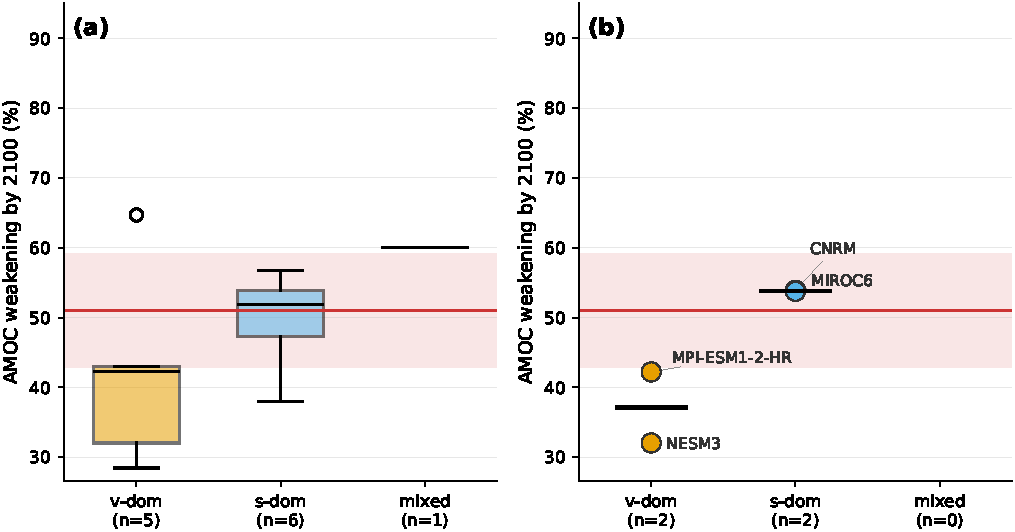
\includegraphics[width=\linewidth]{Figure3.pdf}
\fi
\caption{\textbf{AMOC projections for the bistable-only subset.}
Same as Figure~\ref{fig:cmip6_projection}(c) but restricted to models that are bistable at baseline (\(F_{\mathrm{ovS}}<0\)). Panel~(a) shows the full ensemble for reference; panel~(b) shows only the bistable-baseline subset. The median AMOC weakening remains 52\% for salinity-dominant models (\(n=4\)) and 42\% for velocity-dominant models (\(n=2\)). The persistence of the \(\sim\)10-percentage-point gap rules out the possibility that the mechanism-conditional difference is driven by the well-known CMIP6 fresh bias in the South Atlantic (monostable baseline). Red horizontal line and shaded band: \citet{Portmann2026} constraint.}
\label{fig:bistable_subset}
\end{figure}

\paragraph*{The observed freshening trend is not robust across reanalyses}

The mechanism disagreement between ORAS5 and GLORYS12V1 is striking, but a deeper question remains: is the decline in \(F_{\mathrm{ovS}}\) itself a robust signal? To test this, we repeated the decomposition using only fully post-Argo windows (2006--2012 versus 2018--2024), thereby removing any possible artefact from the pre-Argo observing-system shock. As shown in Figure~\ref{fig:robustness}(a), GLORYS12V1 remains strongly salinity-dominant (\(+90\%\) salinity share), confirming that its attribution to salt redistribution is not a spurious result of the Argo transition. By contrast, ORAS5 shifts from velocity-dominant (89\% velocity share in the main windows) to mixed (44\% velocity share, 57\% salinity share) in the post-Argo windows. This indicates that part of ORAS5's original velocity-driven signal is likely an artefact of the observing-system shock rather than a forced climate trend.

Even more critically, the only 4D-variational product in our ensemble, ECCO-V4r4, exhibits a near-zero change (\(\Delta F_{\mathrm{ovS}} = -2\) mSv, well below the 10 mSv threshold for mechanism classification). ECCO-V4r4 is produced by a long-window adjoint (4D-variational) optimisation that enforces dynamical self-consistency and near-mass-conservation over the full record by iteratively adjusting initial conditions and forcing. Its lack of trend is the dynamically-consistent answer. This null result directly contradicts the large declines seen in ORAS5 (\(-34\) mSv) and GLORYS12V1 (\(-91\) mSv). The disagreement cannot be dismissed as a smoothing artefact; it must either reflect ECCO's weaker assimilation constraints on interior salinity, or indicate that the ORAS5/GLORYS12V1 trends are partially observing-system artefacts. Disentangling these possibilities is a key target for future work.

Taken together, the robustness tests (Figure~\ref{fig:robustness}(b) and (c)) confirm that the mechanism split is real and not a noise artefact, but they also reveal a more profound uncertainty: we cannot be certain that the \(F_{\mathrm{ovS}}\) trend itself is a forced climate signal. While GLORYS12V1's salinity-dominance survives all checks, ORAS5's velocity attribution is partly artefactual, and ECCO's null trend challenges whether any secular decline has actually occurred. Therefore, the community's confidence in AMOC weakening projections must be tempered not only by the mechanism ambiguity but also by the possibility that the observational fingerprint itself is reanalysis-dependent.

% =========================================================================
% Figure 4: Robustness – observing-system shocks, period choice, signal-to-noise
% =========================================================================
\begin{figure}
\centering
\ifsplitfigs
  \begin{subfigure}{\linewidth}\centering
    
\includegraphics[width=\linewidth]{Figure4a.pdf}
    \caption{}\label{fig:f4a}
  \end{subfigure}\\[4pt]
  \begin{subfigure}{0.49\linewidth}\centering
    
\includegraphics[width=\linewidth]{Figure4b.pdf}
    \caption{}\label{fig:f4b}
  \end{subfigure}\hfill
  \begin{subfigure}{0.49\linewidth}\centering
    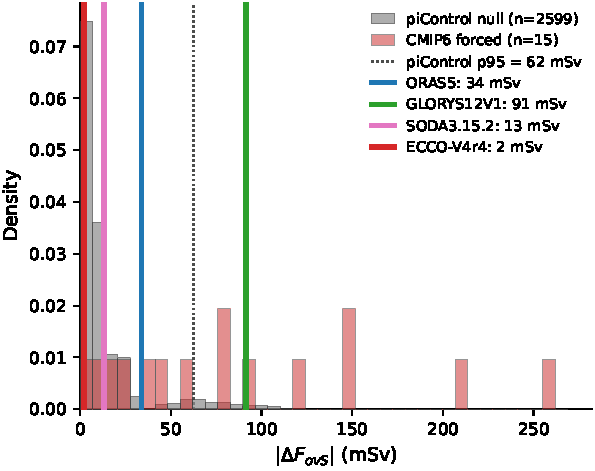
\includegraphics[width=\linewidth]{Figure4c.pdf}
    \caption{}\label{fig:f4c}
  \end{subfigure}
\else
  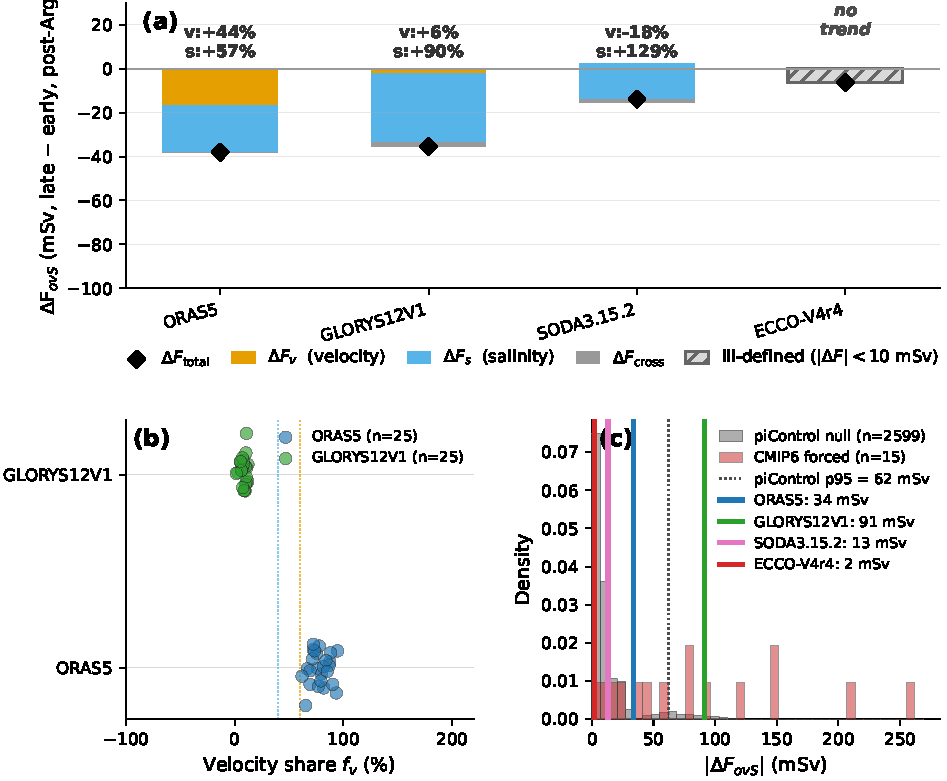
\includegraphics[width=\linewidth]{Figure4.pdf}
\fi
\caption{\textbf{Robustness of the mechanism disagreement.}
\textbf{(a)} Post-Argo robustness test (early 2006--2012 versus late 2018--2024). GLORYS12V1 remains strongly salinity-dominant ($+90\%$ salinity share); ORAS5 shifts from velocity-dominant (in the main windows) to mixed -- indicating part of its signal may be an observing-system shock.
\textbf{(b)} Sensitivity to period choice. Velocity-share ($f_v$) distributions across 25 early/late window pairs. ORAS5 and GLORYS12V1 distributions never overlap -- the mechanism disagreement is robust.
\textbf{(c)} Signal-to-noise test. Histogram of $|\Delta F_{\mathrm{ovS}}|$ from 2600 piControl 30-year segments (internal variability). ORAS5 (31 mSv) and GLORYS12V1 (87 mSv) exceed the 95th percentile (22 mSv), confirming their mechanism attributions are signal-dominated, not noise.}
\label{fig:robustness}
\end{figure}

\paragraph*{Spatial fingerprints confirm opposite mechanisms: western boundary current versus basin-scale salinification}

The decomposition results in Figure~\ref{fig:reanalysis_mechanism} show that ORAS5 and GLORYS12V1 attribute the freshening to fundamentally different processes. To test whether these attributions have distinct spatial expressions, we examine the zonal structure of the velocity and salinity changes at 34.5°S, shown in Figure~\ref{fig:zonal_structure}.

For ORAS5, the large positive velocity anomalies (\(\Delta v\)) are confined to the western boundary current region -- the path of the Brazil Current and the deep western boundary current. This pattern indicates that the change in freshwater transport is driven primarily by an acceleration or structural shift of the boundary current itself, consistent with a wind-driven, circulation-dominant mechanism. In contrast, GLORYS12V1 exhibits a basin-scale positive salinity anomaly (\(\Delta S\)) in the upper 1000 m, extending across most of the Atlantic section. This broad salinification is precisely the "salt-pile-up" signature predicted by salt-advection feedback theory: a slowing overturning accumulates salt in the subtropical gyre, which then amplifies the initial perturbation. No such widespread salinity change is seen in ORAS5.

Thus, the spatial patterns independently confirm that ORAS5's velocity-driven attribution is rooted in local circulation changes, while GLORYS12V1's salinity-driven attribution reflects a basin-integrated redistribution of salt. These distinct fingerprints are consistent with the opposing mechanisms deduced from the vertically integrated decomposition and provide strong observational evidence that the reanalysis disagreement is not a statistical artefact but a real difference in how the Atlantic's freshening is represented.

% =========================================================================
% Figure 5: Zonal structure of velocity and salinity changes
% =========================================================================
\begin{figure}
\centering
\ifsplitfigs
  \begin{subfigure}{0.49\linewidth}\centering
    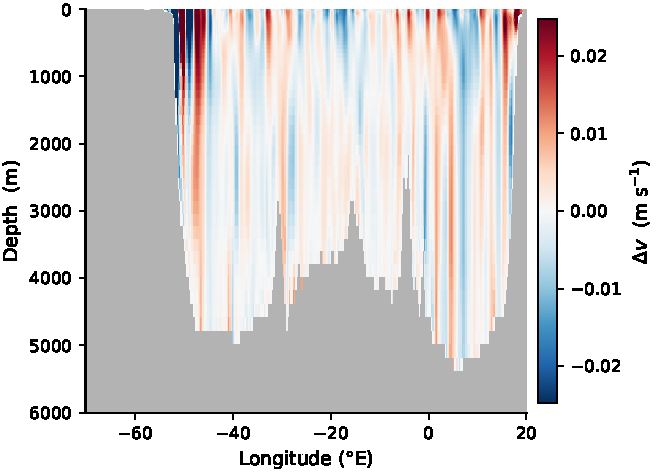
\includegraphics[width=\linewidth]{Figure5a.pdf}
    \caption{}\label{fig:f5a}
  \end{subfigure}\hfill
  \begin{subfigure}{0.49\linewidth}\centering
    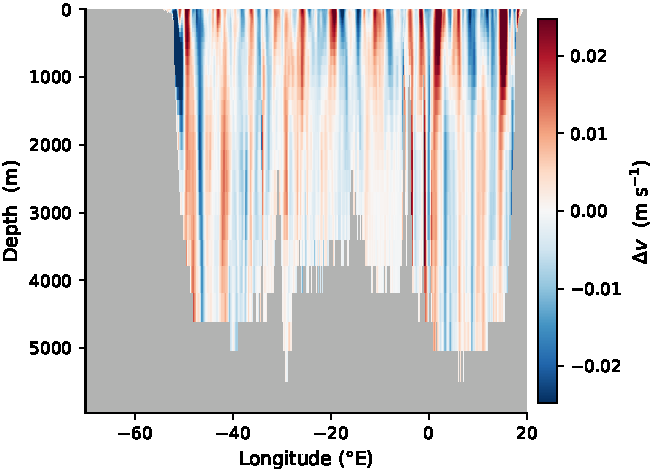
\includegraphics[width=\linewidth]{Figure5b.pdf}
    \caption{}\label{fig:f5b}
  \end{subfigure}\\[4pt]
  \begin{subfigure}{0.49\linewidth}\centering
    
\includegraphics[width=\linewidth]{Figure5c.pdf}
    \caption{}\label{fig:f5c}
  \end{subfigure}\hfill
  \begin{subfigure}{0.49\linewidth}\centering
    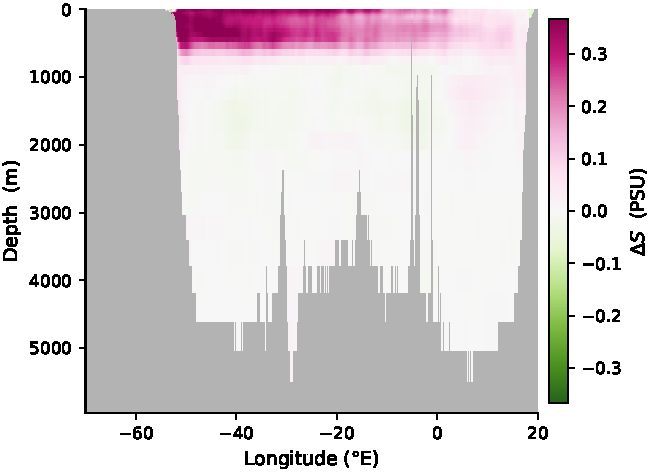
\includegraphics[width=\linewidth]{Figure5d.pdf}
    \caption{}\label{fig:f5d}
  \end{subfigure}
\else
  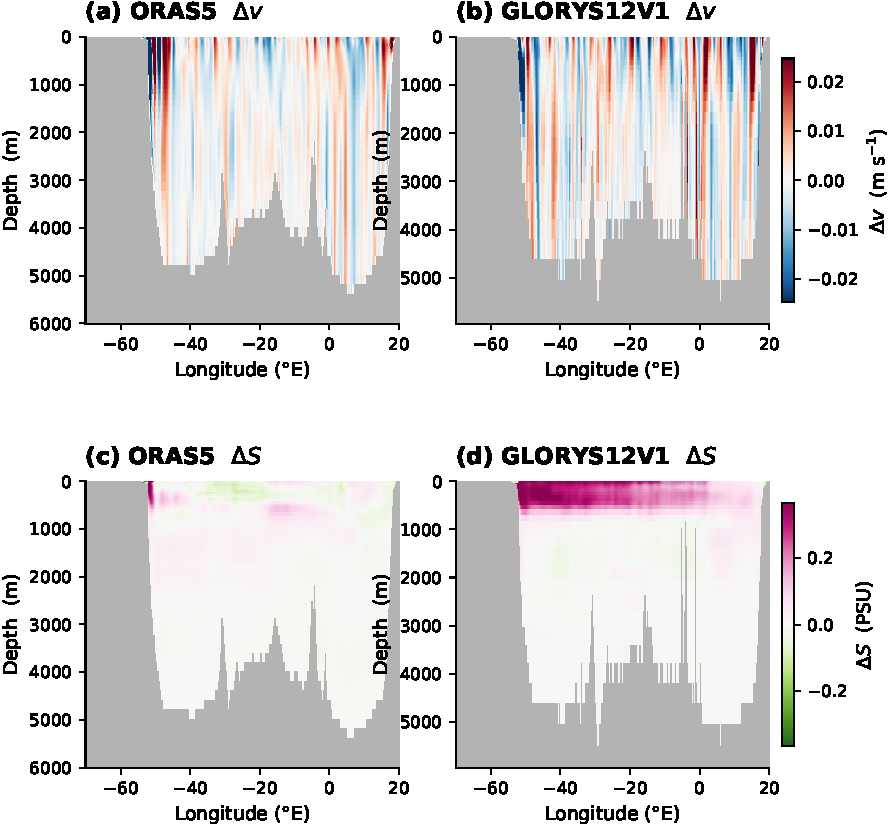
\includegraphics[width=\linewidth]{Figure5.pdf}
\fi
\caption{\textbf{Zonal structure of \(\Delta v\) and \(\Delta S\) at 34.5°S.}
ORAS5 (\textbf{a}, \textbf{c}) shows large velocity changes (\(\Delta v\)) concentrated in the western boundary current region, consistent with a circulation-driven freshening. In contrast, GLORYS12V1 (\textbf{b}, \textbf{d}) displays a basin-scale positive salinity change (\(\Delta S\)) in the upper 1000 m -- the salt-pile-up signature predicted by active salt-advection feedback. Land and sub-bottom topography are shown in grey. Colour scales are saturated at the 95th percentile of the absolute anomaly to highlight basin-scale structure. These distinct spatial patterns provide direct observational evidence for the opposite mechanism attributions shown in Figure~\ref{fig:reanalysis_mechanism}.}
\label{fig:zonal_structure}
\end{figure}

\paragraph*{Barotropic correction removes spurious signals and flags data artefacts}

The decomposition of \(F_{\mathrm{ovS}}\) relies on explicit subtraction of the section-mean (barotropic) velocity to isolate the overturning component. Without this correction, spurious trends arise from non-zero net volume transport across the section, which can reach up to 5 Sv in SODA 3.15.2 (Table~\ref{tab:T1}). The correction removes an artificial signal of 10-40 mSv -- comparable to the \(\Delta F_{\mathrm{ovS}}\) values that define mechanism classification -- and qualitatively changes the attribution for several products.

A striking illustration is the SODA 3.15.2 annual mean for 1998, which under the uncorrected formula gives \(F_{\mathrm{ovS}} = -1.77\) Sv -- an order-of-magnitude outlier caused by a data corruption (salinity as low as 13-17 PSU in some grid cells). After applying the barotropic correction, the 1998 value collapses to -0.018 Sv and no longer qualifies as an outlier. This demonstrates that apparent data artefacts in reanalysis-derived \(F_{\mathrm{ovS}}\) can be artificially inflated when the barotropic subtraction is omitted. All 43 SODA annual values are retained in our analysis, and the correction is applied uniformly across all reanalyses and CMIP6 models, ensuring a consistent and physically meaningful decomposition.

% =========================================================================
% Table: Net volume transport across 34.5°S
% =========================================================================
\begin{table}
\centering
\caption{\textbf{Net volume transport ($V_\mathrm{net}$) across 34.5\textdegree S per product and per decomposition window.} $V_\mathrm{net} = \int V_\mathrm{int}(z)\,\mathrm{d}z$ is the quantity the barotropic subtraction in our $\Fovs$ kernel removes; its magnitude indicates how strongly the product violates depth-integrated mass conservation over the section. Without the subtraction a $|\Delta V_\mathrm{net}|$ drift of 1~Sv between periods would inject approximately $|\Delta V_\mathrm{net}|\cdot|\bar{S}-S_0|/S_0 \approx 14$~mSv of spurious signal into $\Delta\Fovs$. All values reported here are the period-mean $V_\mathrm{net}$ in Sv after the barotropic correction was NOT yet applied to the period average (diagnostic only; the F\_ov computation itself is barotropic-corrected throughout).}
\label{tab:T1}
\small
\begin{tabular}{lrrrr}
\toprule
 & \multicolumn{2}{c}{Main window [Sv]} & \multicolumn{2}{c}{Post-Argo window [Sv]} \\
\cmidrule(lr){2-3} \cmidrule(lr){4-5}
Product & $V_\mathrm{net}$ early & $V_\mathrm{net}$ late & $V_\mathrm{net}$ early & $V_\mathrm{net}$ late \\
\midrule
ORAS5 & $-1.12$ & $-0.82$ & $-1.04$ & $-0.64$ \\
GLORYS12V1 & $-1.39$ & $-0.97$ & $-1.16$ & $-1.07$ \\
SODA 3.15.2 & $-4.00$ & $-3.84$ & $-3.86$ & $-5.02$ \\
ECCO-V4r4 & $-1.25$ & $-1.08$ & $-1.17$ & $-1.11$ \\
\bottomrule
\end{tabular}
\end{table}

\paragraph*{Lead-lag and emergent constraints confirm fingerprint role but miss mechanism split}

Beyond the mechanism disagreement, we examine two supporting diagnostics: the lead-lag relationship between \(F_{\mathrm{ovS}}\) and AMOC strength, and the emergent constraint that uses historical \(F_{\mathrm{ovS}}\) to constrain future AMOC weakening. These analyses, shown in Figure~\ref{fig:f6_diagnostics}, provide additional context for interpreting the reanalysis and CMIP6 results.

First, cross-correlation analysis (Figure~\ref{fig:f6_diagnostics}\textbf{(a)}) reveals that \(F_{\mathrm{ovS}}\) typically leads AMOC variations at 26.5°N by about 5-10 years in most CMIP6 models. This is consistent with the theoretical role of \(F_{\mathrm{ovS}}\) as a fingerprint: changes in freshwater export precede adjustments in the overturning strength. The lead time varies across models, but the sign is robust -- \(F_{\mathrm{ovS}}\) is a leading indicator, not a passive response.

Second, the emergent constraint (Figure~\ref{fig:f6_diagnostics}\textbf{(b)}) plots historical \(F_{\mathrm{ovS}}\) (2000-2024) against end-of-century \(F_{\mathrm{ovS}}\) under SSP5-8.5. The observed value of \(-0.078 \pm 0.024\) Sv (derived from the reanalysis mean) lies within the range of the CMIP6 models and, when projected forward, narrows the 95\% forecast interval relative to the unconstrained CMIP6 ensemble. However, this emergent constraint does not distinguish between velocity-dominant and salinity-dominant models. The spread in the projection is large, and -- crucially -- the constraint does not account for the mechanistic split identified in this study. Consequently, the emergent method overestimates the confidence in its central estimate by implicitly averaging over the two opposing mechanisms.

Taken together, these supporting analyses reinforce the value of \(F_{\mathrm{ovS}}\) as a leading indicator but also expose a more fundamental limitation of single-variable emergent constraints in this CMIP6 ensemble: F$_{\mathrm{ovS}}$ at 2000--2024 is too weakly correlated with $\Delta\mathrm{AMOC}_{26^\circ\mathrm{N}}$ over 2030--2040 (R\textsuperscript{2}~$\approx$~0.01) for any pooled or class-conditional regression to deliver a tight forecast. This is consistent with -- not contradictory to -- our central thesis. The 10-percentage-point AMOC-weakening gap (Fig.~\ref{fig:cmip6_projection}) is recovered by conditioning on the underlying \emph{physics} (the mechanism class) rather than by leveraging F$_{\mathrm{ovS}}$ as a regression predictor. The emergent-constraint regression therefore complements rather than competes with the mechanism partition; both point to the same conclusion -- that the inter-model spread is structured by physics that any one-dimensional constraint must average over (Supplementary Fig.~S5).

% =========================================================================
% Figure 6: Diagnostics + SMILE robustness (formerly Fig 6 + Fig 7)
% =========================================================================
\begin{figure}
\centering
\ifsplitfigs
  \begin{subfigure}{0.49\linewidth}\centering
    
\includegraphics[width=\linewidth]{Figure6a.pdf}
    \caption{}\label{fig:f6a}
  \end{subfigure}\hfill
  \begin{subfigure}{0.49\linewidth}\centering
    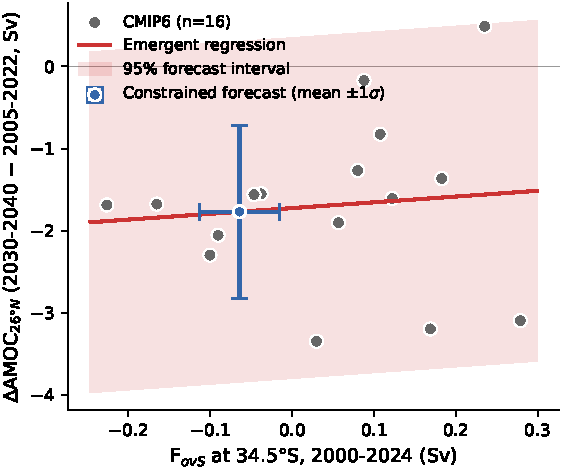
\includegraphics[width=\linewidth]{Figure6b.pdf}
    \caption{}\label{fig:f6b}
  \end{subfigure}\\[0.6em]
  \begin{subfigure}{0.49\linewidth}\centering
    
\includegraphics[width=\linewidth]{Figure6c.pdf}
    \caption{}\label{fig:f6c}
  \end{subfigure}\hfill
  \begin{subfigure}{0.49\linewidth}\centering
    
\includegraphics[width=\linewidth]{Figure6d.pdf}
    \caption{}\label{fig:f6d}
  \end{subfigure}
\else
  
\includegraphics[width=\linewidth]{Figure6.pdf}
\fi
\caption{\textbf{Diagnostic relationships and SMILE robustness of the mechanism classification.}
\textbf{(a)} Cross-correlation curves between $F_{\mathrm{ovS}}$ and AMOC for individual CMIP6 models (positive lag $\tau$ = $F_{\mathrm{ovS}}$ leads AMOC). Solid red: collapsing-class ensemble mean ($\pm 1\sigma$ ribbon). Dashed blue: stable-class ensemble mean. Most models show $F_{\mathrm{ovS}}$ as a leading indicator.
\textbf{(b)} CMIP6 emergent regression of $F_{\mathrm{ovS}}$ at 34.5°S (2000-2024) against $\Delta\mathrm{AMOC}_{26^\circ\mathrm{N}}$ over the 2030-2040 forecast window. Slope $a = +0.70$, intercept $b = -1.73$, $R^2 = 0.01$, $\sigma_\mathrm{res} = 1.05$~Sv. Blue band: observational $F_{\mathrm{ovS}}$ ($-0.078\pm0.024$~Sv) propagated through the regression; the resulting constrained forecast $\Delta\mathrm{AMOC} = -1.77$~Sv (95\% CI $[-3.83, +0.29]$) is essentially identical to the unconstrained CMIP6 mean. Partitioning the regression by mechanism class does not recover predictive power either (within-class $R^2 \le 0.11$; Supplementary Fig.~S5). The 10-percentage-point AMOC-weakening gap visible in Figure~\ref{fig:cmip6_projection}\textbf{(c)} therefore arises from the mechanism-class partition itself rather than from any direct $F_{\mathrm{ovS}}$--AMOC regression.
\textbf{(c)} F$_{\mathrm{ovS}}$ velocity-share ($f_v$) vs salinity-share ($f_s$) for all 50 initial-condition members of the MPI-ESM1-2-LR Grand Ensemble (orange crosses), overlaid on the multi-model CMIP6 ensemble (faded coloured circles). The black diamond marks the SMILE ensemble mean. Vertical and horizontal dotted lines mark the $f_v=60\%$ and $f_s=60\%$ classification thresholds; dashed grey line: $f_v+f_s=100\%$. All 50 SMILE members fall in the velocity-dominant quadrant (mean $f_v=+93\%$, $\sigma=15\%$, minimum $f_v=+73\%$); the 60\% threshold sits $2.2\sigma$ below the cluster mean.
\textbf{(d)} AMOC time series at 26.5°N (max of $\mathtt{msftmz}$ below 500~m, the standard RAPID-equivalent definition) for all 50 SMILE members, 1850-2100, hist+ssp585. Orange spaghetti: per-member trajectories. Dark-orange line: ensemble mean. Orange envelope: $\pm 1\sigma$ across members. Vertical dashed line: hist$\rightarrow$ssp585 transition (2014). Grey vertical bands: the 1950-1980 baseline and 2081-2100 forced windows used for percent-weakening. 1950-1980 ensemble-mean AMOC = $+18.8\pm 0.4$~Sv (1$\sigma$); 2081-2100 ensemble-mean AMOC = $+14.4\pm 0.3$~Sv; per-member weakening = $+23.3\%\pm 2.4\%$ (1$\sigma$), range $[+18\%,+29\%]$.}
\label{fig:f6_diagnostics}
\end{figure}

\paragraph*{Single-model large-ensemble robustness rules out internal-variability aliasing}

A reasonable concern with the binary mechanism classification of single-realisation CMIP6 models is that the assigned class -- velocity-dominant vs salinity-dominant -- might be partly an artefact of the phase of internal variability sampled by the \texttt{r1i1p1f1} realisation, rather than a structural property of the model. We address this directly using the 50-member MPI-ESM1-2-LR Grand Ensemble downloaded via DKRZ ESGF: every member shares identical model code, parameterizations and forcing, and only the initial-condition perturbation differs. As shown in Figure~\ref{fig:f6_diagnostics}, all 50 members fall in the velocity-dominant quadrant of the F$_{\mathrm{ovS}}$ decomposition plane (panel~\textbf{(c)}; ensemble-mean $f_v=+93\%$, standard deviation $\sigma=15\%$; the $60\%$ classification threshold sits $2.2\sigma$ below the cluster mean), and the AMOC weakening at 26.5°N (panel~\textbf{(d)}) clusters tightly across all 50 members (ensemble-mean weakening $+23.3\%$ by 2100, $\sigma=2.4$ percentage points; range $[+18\%,+29\%]$). The internal-variability spread on the projected weakening is therefore $\sim$4$\times$ smaller than the multi-model 10-percentage-point gap reported in Figure~\ref{fig:cmip6_projection}\textbf{(c)}, confirming that the mechanism-class assignment is set by structural physics -- chiefly the model's coupled wind-driven Southern-Hemisphere response and NADW-formation sensitivity (Discussion) -- rather than by a particular phasing of decadal variability.

\section*{Discussion}

Our findings isolate a fundamental ambiguity in ocean reanalysis representations of Atlantic freshening. All four evaluated products identify a negative \(F_{\mathrm{ovS}}\), confirming the bistable regime, yet they diverge drastically on the underlying physics driving the recent decline. ORAS5 isolates circulation shifts (velocity-driven), whereas GLORYS12V1 captures a basin-scale salt redistribution (salinity-driven)—the precise fingerprint of an active salt-advection feedback. The implications for AMOC stability are severe: wind-forced velocity trends remain largely reversible, presenting little evidence of an imminent tipping point. Conversely, a salinity-driven trend signals that the salt-advection feedback operates actively, exacerbating the risk of convection collapse in the subpolar North Atlantic.

This mechanistic divergence persists in CMIP6 forced-weakening simulations \citep{Sgubin2017, IPCC_AR6_Chapter9}. The models bifurcate into distinct salinity-dominant and velocity-dominant clusters, with the reanalysis end-members bounding the distribution. This spread reflects structural physical diversity, not a transient reanalysis anomaly. Conditioning future AMOC trajectories on the underlying mechanism exposes a stark gap: salinity-dominant models project a median 2100 weakening of 52\%, aligning tightly with the emergent-constraint estimate of \citet{Portmann2026}, while velocity-dominant models project a milder 42\% decline. Current observational constraints implicitly average over this mechanism dimension, systematically underestimating uncertainty—a vulnerability increasingly recognized across the AMOC literature \citep{RahmstorfCaesar2026}.

Stringent robustness tests reinforce this division. The salinity-dominant signature in GLORYS12V1 withstands post-Argo filtering, proving it transcends observing-system shocks. In contrast, the velocity-dominant signal in ORAS5 deteriorates into a mixed state during the post-Argo era, suggesting residual data-assimilation artifacts. Further complicating the consensus, ECCO-V4r4—the only 4D-variational adjoint state estimate—exhibits a near-zero trend. This dynamically consistent trajectory directly challenges the steep declines mapped by ORAS5 and GLORYS12V1, rendering the existence of a forced secular freshening trend observationally uncertain.

The velocity-vs-salinity dichotomy we identify in $F_{\mathrm{ovS}}$ at 34.5°S is consistent with -- and most parsimoniously interpreted through -- the wind-vs-buoyancy split documented in recent CMIP6 AMOC-attribution studies. \citet{Asbjornsen2023} decompose future AMOC decline at 26.5°N into Gulf Stream, deep western boundary current (DWBC) and gyre-recirculation contributions, finding that approximately one-third of the projected Gulf Stream weakening is driven by wind-stress curl changes (Sverdrup-theory consistent) while two-thirds compensate for the buoyancy-driven DWBC reduction. \citet{Levang2020} reach a similar conclusion for CMIP5: the geostrophic component of AMOC weakening at 40°N is dominated by temperature anomalies in the 1000--2000 m layer rather than by salinity. \citet{Baker2023} show that the spread in projected AMOC weakening across 27 CMIP6 models (29--61\% by 2100 under SSP5-8.5) is controlled by inter-model differences in the partitioning of the overturning return pathway between the Indo-Pacific and the Southern Ocean. These three lines of evidence motivate a physical reading of our mechanism classes. The velocity-dominant CMIP6 subset (CESM2, FIO-ESM-2-0, MPI-ESM1-2-LR, MPI-ESM1-2-HR, NESM3) is most naturally interpreted as the family of models in which the Southern-Hemisphere wind-driven response dominates the F$_{\mathrm{ovS}}$ change -- consistent with our observation that ORAS5's velocity anomaly is concentrated at the western boundary current (Fig.~5\textbf{(a)}), the locus of Sverdrup gyre adjustment. The salinity-dominant subset (CNRM-CM6-1, FGOALS-g3, GFDL-CM4, HadGEM3-GC31-LL, MIROC6, UKESM1-0-LL) corresponds to models in which the buoyancy-driven NADW reduction propagates south as a basin-wide upper-1000-m salinity redistribution at 34.5°S -- the salt-pile-up signature predicted by salt-advection-feedback theory \citep{Stommel1961, deVriesWeber2005}, visible in GLORYS12V1's spatial pattern (Fig.~5\textbf{(d)}). The 50-member MPI-ESM1-2-LR Grand Ensemble (Figure~\ref{fig:f6_diagnostics}\textbf{(c,d)}) corroborates this physical reading: 50 of 50 initial-condition members cluster tightly in the velocity-dominant quadrant ($f_v$ mean $+93\%$, $\sigma = 15\%$, minimum $73\%$ -- the classification threshold of $60\%$ sits $2.2\sigma$ below the cluster mean), confirming that MPI-ESM1-2-LR's mechanism class is set by its wind-driven Southern-Ocean response physics rather than by an arbitrary realisation of internal variability.

We acknowledge specific methodological limits. The diagnostic decomposition relies on statistical integration rather than exact physical causality; the velocity and salinity fields remain dynamically coupled. Furthermore, internal variability within single-realization CMIP6 projections inevitably aliases the structural signals, and the classification thresholds, while robust to perturbation, remain heuristic.

Nevertheless, these findings enforce a stringent condition on future AMOC constraints. Projections calibrated against historical reanalyses must explicitly incorporate the reanalysis-dependent mechanism. The alignment between the salinity-dominant CMIP6 subset and existing constraints \citep{Portmann2026} indicates an implicit physical selection. Elevating this to an explicit metric—for instance, formally assimilating the zonally-integrated \(\Delta S\) anomaly—will rigorously define projection uncertainties.

Resolving this mechanistic deadlock demands targeted observation. While the SAMBA array at 34.5°S successfully resolves velocity-weighted overturning, it inherently convolves velocity and salinity variations. Securing the predictive foundations of AMOC stability requires deploying a basin-wide salinity repeat-section array in the South Atlantic, parallel to the OSNAP initiative in the subpolar North Atlantic \citep{Lozier2019, FrajkaWilliams2019}. Without such directed measurements, projections rooted in the \(F_{\mathrm{ovS}}\) fingerprint embed an unresolved \(\sim\)10-percentage-point uncertainty. This gap transcends simple measurement error; it exposes a structural deficit in our grasp of the forces governing Atlantic freshening.

\noindent\textbf{Competing interests}: The authors declare no competing financial or non-financial interests.

\section*{Methods}
\linenumbers

\subsection*{Observational reanalysis datasets}

Four independent global ocean reanalysis products are analysed. They were selected to span the four mainstream data-assimilation paradigms in the global-ocean reanalysis ecosystem -- 3D-Var FGAT (ORAS5), reduced-order Kalman filter with 3D-Var bias correction (GLORYS12V1), ensemble optimal interpolation (SODA 3.15.2), and 4D-variational adjoint state estimation (ECCO-V4r4) -- and together cover the eddy-resolving ($1/12^\circ$) to coarse-resolution ($1/2^\circ$) range used in CMIP-class climate analysis. This is the same four-product canonical ensemble adopted by the headline emergent-constraint study \citep{Portmann2026}, ensuring that our mechanism decomposition is directly comparable to that constraint without product-selection ambiguity. Adding a fifth product from any of the same paradigms (e.g.~ORAS4, C-GLORS, FOAM) would not break the velocity-vs-salinity dichotomy because such siblings share systematic biases with their corresponding family member; a complementary GECCO3 (Hamburg) 4D-Var run would be the most informative future addition because it would test whether the ECCO null trend is generic to adjoint optimisation. The four products together represent the currently available space of observationally-constrained three-dimensional ocean state estimates at 34.5$^\circ$S.

\paragraph{ORAS5} \citep{Zuo2019}. Ocean Reanalysis System 5 from ECMWF. Native grid: ORCA025 tripolar (nominal $\sim$1/4$^\circ$, $\sim$25~km at the equator and $\sim$14~km at 34.5$^\circ$S after the $\cos\phi$ contraction), 75 vertical levels with 1-m surface resolution. NEMOVAR 3D-Var FGAT data-assimilation scheme ingesting sub-surface temperature/salinity profiles, sea-ice concentration, and along-track altimetric sea-level anomalies. Atmospheric forcing: ERA-40 (1958--1978) transitioning to ERA-Interim/ERA5 (1979--present). Record used: 816 monthly means, 1958--2025.

\paragraph{GLORYS12V1} \citep{Lellouche2021}. Copernicus Marine Service/Mercator Ocean global ocean reanalysis at 1/12$^\circ$ ($\sim$8~km, eddy-resolving), 50 vertical levels. A reduced-order Kalman filter (SAM2) jointly assimilates along-track altimetry, satellite sea-surface temperature, sea-ice concentration, and in-situ CTD and Argo temperature/salinity profiles, supplemented by 3D-Var bias correction. Atmospheric forcing: ERA5. Record used: 396 monthly means, 1993--2025 (satellite-altimetry era).

\paragraph{SODA 3.15.2} \citep{Carton2018}. Simple Ocean Data Assimilation 3 from the University of Maryland. Native grid: MOM5 $\sim$1/2$^\circ$ (regridded to a uniform 0.5$^\circ$ product on the UMD mirror), 50 vertical levels. Assimilation scheme: ensemble optimal interpolation with a 5-day analysis cycle; the downloadable output is a sequence of 5-day snapshots. Atmospheric forcing: MERRA-2. We sample four 5-day snapshots per year (mid-month of January, April, July, October) to approximate the annual mean, consistent with previous applications of the same product to overturning-transport diagnostics. Record used: 43 annual means, 1980--2022.

\paragraph{ECCO-V4r4} \citep{Forget2015}. NASA/JPL Estimating the Circulation and Climate of the Ocean, version 4 release 4. Native grid: LLC90 Lat-Lon-Cap (regridded to a uniform 0.5$^\circ$ monthly product), 50 vertical levels. ECCO is an adjoint-based least-squares state estimate (4D-variational) that iteratively adjusts initial conditions, surface fluxes, and interior mixing to minimise the misfit between the model trajectory and the full suite of altimetry, Argo, satellite SST/SSH, and mooring observations over its full time span. Atmospheric forcing (post-iteration): an ECCO-adjusted ERA-family atmospheric analysis. Record used: 26 annual means, 1992--2017.

\paragraph{Direct-hydrography anchors.} Three published overturning freshwater-transport estimates at 34.5$^\circ$S from direct in-situ observations are used as independent anchor points in Fig.~1: \citet{GarzoliMatano2011} (central year 2005, value $-0.10\pm0.10$~Sv); \citet{Meinen2018} (central year 2015, value $-0.09\pm0.05$~Sv); and \citet{Kersale2020} (central year 2015, value $-0.17\pm0.07$~Sv). Together with \citet{ArumiPlanas2024}'s $-0.15\pm0.09$~Sv from 49 XBT transects, they bracket the reanalysis ensemble from the low side.

\subsection*{CMIP6 ensemble}

CMIP6 meridional-velocity (\texttt{vo}) and salinity (\texttt{so}) sections at 34.5$^\circ$S are obtained for every available model with coverage of both the \texttt{historical} experiment (required period 1950--1980) and the \texttt{ssp585} experiment (required period 2080--2100). The native grid of each model is used (i.e. no regridding), because regridding distorts the mechanistic decomposition. Fifteen models satisfy both criteria with accessible section files: CESM2, CMCC-CM2-SR5, CNRM-CM6-1, CanESM5, FGOALS-g3, FIO-ESM-2-0, GFDL-CM4, GISS-E2-1-G, HadGEM3-GC31-LL, IPSL-CM6A-LR, MIROC6, MPI-ESM1-2-HR, MPI-ESM1-2-LR, NESM3, UKESM1-0-LL. Three models are excluded: NorESM2-LM and NorESM2-MM because their ocean component is on isopycnal (density) coordinates and cannot be integrated in depth-space without an additional remap that would confound the decomposition; and ACCESS-CM2 because its accessible \texttt{ssp585} run does not extend to 2100. All models use the \texttt{r1i1p1f1} realisation.

A 13-model subset with \texttt{piControl} access is used for the internal-variability null test: ACCESS-CM2, CESM2, CMCC-CM2-SR5, CNRM-CM6-1, CanESM5, GISS-E2-1-G, HadGEM3-GC31-LL, IPSL-CM6A-LR, MIROC6, MPI-ESM1-2-HR, MPI-ESM1-2-LR, NESM3, UKESM1-0-LL.

\paragraph{Ensemble size used per analysis.} Different downstream analyses retain different subsets of the 15-model decomposition ensemble:

\begin{itemize}
\item \emph{Mechanism decomposition + tiebreaker scatter} (Figs.~1b, 2a of the main text): all 15 models. Three models are flagged \emph{increasing} (CMCC-CM2-SR5, CanESM5, IPSL-CM6A-LR) and excluded from the mechanism-conditional projection because their forced $\Fovs$ change is positive; this leaves \textbf{12 weakening models} that drive the headline 10-percentage-point gap (Figs.~2b,~2c).
\item \emph{Bistable-only subset} (Fig.~3): 6 models have $\overline{\Fovs}(t_1)<0$; of those, 2 are \emph{increasing} and are dropped, leaving \textbf{$n=4$ weakening + bistable} models (CNRM-CM6-1, MIROC6 salinity-dominant; MPI-ESM1-2-HR, NESM3 velocity-dominant).
\item \emph{piControl null} (Fig.~4c): \textbf{13 models} (the subset listed above), with up to 200 random non-overlapping 30-year window pairs per model.
\item \emph{Lead-lag cross-correlation} (Fig.~6a) and \emph{emergent constraint regression} (Fig.~6b): \textbf{16 models}. Both diagnostics use only the 1850-2024 historical+\texttt{ssp585} window for the lead-lag and the 2000-2024 / 2030-2040 windows for the emergent constraint, which means ACCESS-CM2 -- excluded from the decomposition because its \texttt{ssp585} run does not reach 2100 -- can be retained here. We re-add it to maximise statistical power on the lead-lag cross-correlation function and on the regression slope.
\end{itemize}

This per-analysis bookkeeping is reflected in each figure's panel-internal $n=$ labels and in the captions of the main text.

\subsection*{Section extraction and grid metrics}

At each time step of each product we extract the zonal-depth section at the gridded latitude closest to $-34.5^\circ$. Where the ocean-model grid is staggered (e.g. velocity at U-points and salinity at T-points on the ORAS5 NEMO grid), the two fields are extracted on their native grids and aligned by truncation to the common Atlantic-longitude mask.

The Atlantic basin at 34.5$^\circ$S is defined by the longitude range $[-70^\circ, 20^\circ]$ in the $[-180^\circ, 180^\circ]$ convention (bounds chosen inclusively to cover from the Argentine coast to the African coast while excluding residual Agulhas leakage; the small $<1\%$ contribution from the strictly-classified Drake-Passage edge does not alter the results).

The zonal grid spacing at each Atlantic U-point is
\[
\Delta x_i = |\Delta\lambda_i|\, R_\oplus\, \cos\phi,
\]
with $\Delta\lambda_i$ the local longitudinal grid spacing (after longitude wrap-around correction), $R_\oplus = 111$~km per degree at the equator, and $\phi = -34.5^\circ$. Vertical cell thicknesses $\Delta z_k$ are taken directly from the product's vertical coordinate (with the CESM-family POP grid converted from centimetres to metres).

\subsection*{$\Fovs$ computation}

We follow the definition of \citet{deVriesWeber2005}, used also by \citet{Dijkstra2007, Drijfhout2011, vanWesten2024}:
\[
\Fovs = -\frac{1}{S_0}\int_{z_\mathrm{bot}}^{z_\mathrm{surf}}
  V_\mathrm{int}(z)\,[\bar{S}(z) - S_0]\,\mathrm{d}z,
\]
with
\[
V_\mathrm{int}(z) = \sum_{i\in\mathrm{Atl}} v(x_i, z)\,\Delta x_i \qquad(\mathrm{m}^2/\mathrm{s}),
\]
and
\[
\bar{S}(z) = \frac{\sum_{i\in\mathrm{Atl}} S(x_i, z)\,\Delta x_i
                  \cdot m(x_i, z)}
                 {\sum_{i\in\mathrm{Atl}} \Delta x_i \cdot m(x_i, z)},
\]
where $m(x_i, z)\in\{0, 1\}$ is the wet-cell mask (unity over the ocean, zero over bathymetry). The reference salinity is fixed at $S_0 = 35$~PSU throughout. The integral is evaluated by a discrete sum over vertical levels using the native $\Delta z_k$ as quadrature weights; the final result is reported in Sverdrups (Sv = $10^6~\mathrm{m}^3/\mathrm{s}$). This kernel is implemented once in \texttt{ardp/physics/fovs.py} and reused for every product (reanalyses, CMIP6 historical/ssp585, piControl) to eliminate cross-product inconsistencies.

\subsubsection*{Barotropic-velocity subtraction}

$\Fovs$ is, by construction, the freshwater transport carried by the zonally-averaged \emph{overturning} (baroclinic) circulation, i.e. the component with $\int V_\mathrm{int}(z)\,\mathrm{d}z = 0$ across the section. In a mass-conserving model the net volume transport through a zonal section is exactly zero, so this constraint is satisfied automatically. Data-assimilating Boussinesq reanalyses (ORAS5, GLORYS12V1, SODA~3.15.2, ECCO-V4r4) and Boussinesq coupled models in CMIP6, however, do \emph{not} enforce volume conservation across an arbitrary zonal section, and their net transport $V_\mathrm{net} = \int V_\mathrm{int}(z)\,\mathrm{d}z$ generally takes non-zero values that drift slowly between months and decades as data-assimilation increments or parameterised surface sources re-balance the basin. If this drift is left in, it couples to the offset $\bar{S}(z) - S_0$ and injects a spurious mSv-scale signal into $\Fovs$ that has nothing to do with the overturning.

We therefore follow \citet{deVriesWeber2005, Mecking2017, Weijer2019} and explicitly subtract the section-mean (barotropic) velocity
\[
\bar{v}_\mathrm{bt} \equiv
   \frac{\int V_\mathrm{int}(z)\,\mathrm{d}z}
        {\int A_{xy}(z)\,\mathrm{d}z},
  \qquad
A_{xy}(z) \equiv \sum_{i\in\mathrm{Atl}} \Delta x_i\,m(x_i, z),
\]
before evaluating $\Fovs$, replacing $V_\mathrm{int}(z)$ by its baroclinic residual $V_\mathrm{int}^{\mathrm{bc}}(z) \equiv V_\mathrm{int}(z) - \bar{v}_\mathrm{bt}\,A_{xy}(z)$. By construction, $\int V_\mathrm{int}^{\mathrm{bc}}(z)\,\mathrm{d}z \equiv 0$, which eliminates the volume-drift artefact. The subtraction is applied independently to each monthly snapshot of each product (so the correction tracks the DA increments in time) and is enforced identically on all four reanalyses, on all CMIP6 models, and on the \texttt{piControl} null ensemble.

Across the two decomposition windows reported here the magnitude of $V_\mathrm{net}$ is $\sim0.9$--$1.4$~Sv for ORAS5 and GLORYS12V1, $\sim1.1$--$1.3$~Sv for ECCO-V4r4, and $\sim3.8$--$5.0$~Sv for SODA 3.15.2 (see Table~1 in main text); the $\sim10$--$40$~mSv spurious contribution that the correction removes is therefore of the same order as the $|\Delta\Fovs|$ signals that drive the mechanism classification, and its omission would have qualitatively flipped the classification in several cases. An independent unit test in \texttt{tests/test\_fovs\_decomposition.py} verifies the $\Delta\Fovs = 0$ identity for a pure uniform-velocity drift between two periods.

\subsection*{Mechanism decomposition}

Define $\Delta\Fovs \equiv \Fovs(t_2) - \Fovs(t_1)$ for two non-overlapping period averages $t_1$ (``early'') and $t_2$ (``late''). Writing $v_2 \equiv v_1 + \Delta v$ and $\bar{S}_2 \equiv \bar{S}_1 + \Delta\bar{S}$ and substituting into the definition of $\Fovs$ gives the exact identity
\[
\Delta \Fovs = \dFv + \dFs + \dFc,
\]
where
\[
\begin{aligned}
\dFv &= -\frac{1}{S_0}\int \Delta V_\mathrm{int}(z)\,
        [\bar{S}_1(z) - S_0]\,\mathrm{d}z,\\[2pt]
\dFs &= -\frac{1}{S_0}\int V_{\mathrm{int},1}(z)\,
        \Delta\bar{S}(z)\,\mathrm{d}z,\\[2pt]
\dFc &= -\frac{1}{S_0}\int \Delta V_\mathrm{int}(z)\,
        \Delta\bar{S}(z)\,\mathrm{d}z.
\end{aligned}
\]
$\dFv$ is the change that would have occurred if only the velocity field had changed (salinity frozen at its $t_1$ value); $\dFs$ is the change that would have occurred if only the zonal-mean salinity had changed (velocity frozen at $t_1$); and $\dFc$ is the cross (``eddy'') term that is zero when $\Delta v$ and $\Delta\bar{S}$ are exactly orthogonal in a depth-integrated sense and becomes large and signed when the two anomalies are correlated in $z$. The identity is exact up to floating-point round-off; unit tests verify residual magnitudes of $\mathcal{O}(10^{-15})$~Sv across randomised synthetic sections, velocity-only perturbations, salinity-only perturbations, and land-masked cases.

The \emph{velocity share} and \emph{salinity share} reported throughout are
\[
f_v \equiv 100\cdot \dFv/\Delta\Fovs,\qquad
f_s \equiv 100\cdot \dFs/\Delta\Fovs,\qquad
f_c \equiv 100\cdot \dFc/\Delta\Fovs,
\]
with the exact constraint $f_v + f_s + f_c = 100\%$. An individual share can exceed $100\%$ or be negative whenever the three components do not all carry the same sign. This occurs naturally in the salt-advection-feedback regime when $\Delta v$ and $\Delta\bar{S}$ are anti-correlated in the vertical (e.g. a slowed upper-limb circulation combined with a freshened subtropical layer); then $\dFc$ becomes large and of opposite sign to $\dFv + \dFs$, so that $|f_v|$ and $|f_s|$ each exceed $100\%$. Values $|f_v| > 100\%$ therefore indicate a physically meaningful cross-term, not a numerical artefact.

The decomposition becomes numerically ill-conditioned when $|\Delta\Fovs|$ is small relative to $|\dFv|$, $|\dFs|$, or $|\dFc|$. We pre‑registered a threshold of $|\Delta\Fovs| \ge 10$~mSv below which the mechanism decomposition is declared \emph{ill-defined}. ECCO-V4r4 is the only reanalysis flagged under this rule.

\subsection*{Period choice}

The early and late periods were pre‑registered before processing the fourth reanalysis (SODA 3.15.2): $t_1 = 1993$--$2005$ and $t_2 = 2013$--$2025$. These are the longest non-overlapping windows fully within the common GLORYS12V1 record, avoiding the first few years of the satellite-altimetry era (pre‑1993) while preserving a $\gtrsim10$-year separation. For products with shorter records we use the nearest-in-length late window: SODA 3.15.2 uses $t_2 = 2013$--$2020$; ECCO-V4r4 uses $t_2 = 2013$--$2017$. For CMIP6 we pair historical 1950--1980 against \texttt{ssp585} 2080--2100 to maximise the forced signal-to-noise ratio.

The sensitivity of the classification to the period choice is reported in Fig.~4\textbf{(b)} of the main text by repeating the computation across a grid of $(t_{1,\mathrm{end}}, t_{2,\mathrm{start}})$ pairs ($t_{1,\mathrm{end}}\in\{2001,2003,2005,2007,2009\}$, $t_{2,\mathrm{start}}\in\{2011,2013,2015,2017,2019\}$, always with $t_{1,\mathrm{start}}=1993$ and $t_{2,\mathrm{end}}$ at each product's data end). The resulting 25-point distribution of $f_v$ values is reported per product.

\subsection*{Baseline regime classification}

Beyond the mechanism decomposition, each product and CMIP6 model is classified by its \emph{baseline} regime at the $t_1$ window: \emph{bistable} if $\overline{\Fovs}(t_1) < 0$ (salt-advection feedback active, \citet{Rahmstorf1996}) or \emph{monostable} if $\overline{\Fovs}(t_1) > 0$. This matters because the salt-advection feedback is not physically active in the monostable regime, so a mechanism-classification result from a monostable CMIP6 model is not directly comparable to an observational reanalysis in which the Atlantic is bistable. In our ensemble 6/15 CMIP6 models are bistable at baseline (CNRM-CM6-1, CanESM5, IPSL-CM6A-LR, MIROC6, MPI-ESM1-2-HR, NESM3); 9/15 are monostable — the well-known ``CMIP6 fresh bias'' at the South Atlantic \citep{Mecking2017, Weijer2019, Portmann2026}.

\subsection*{Trend significance}

Annual-mean $\Fovs$ time series are analysed for linear trends under three complementary methods, with a pre‑registered conservative rule that a trend is declared significant only if $p<0.05$ under all three:

\begin{enumerate}
\item \textbf{Naive OLS.} Standard ordinary least-squares regression with residual-variance-based $p$-value, no autocorrelation correction. Reported as the upper-bound significance claim.
\item \textbf{\citet{Santer2000} $N_\mathrm{eff}$.} The residual lag-1 autocorrelation $r_1$ is computed from the OLS residuals of the detrended series. The effective sample size is $N_\mathrm{eff} = N\,(1-r_1)/(1+r_1)$; the trend's standard error is multiplied by $\sqrt{N/(N_\mathrm{eff}-2)}$ and the adjusted $p$-value uses the Student-$t$ distribution with $N_\mathrm{eff}-2$ degrees of freedom. We clip $r_1$ to $[-0.99,0.99]$ for numerical stability.
\item \textbf{GLS Prais-Winsten AR(1).} The series is pre-whitened using a first-order autoregressive estimate of the residual autocorrelation (iterated Prais-Winsten), then the transformed series is fit by OLS; the resulting trend estimate and standard error explicitly account for AR(1) residual correlation.
\end{enumerate}

\subsection*{Mechanism classification rule}

A product is labelled \emph{velocity-dominant} if $f_v > 60\%$, \emph{salinity-dominant} if $f_s > 60\%$, \emph{mixed} if both $f_v \le 60\%$ and $f_s \le 60\%$, and \emph{ill-defined} (no classification) if $|\Delta\Fovs| < 10$~mSv. The $60\%$ threshold and the $10$~mSv floor are pre‑registered and are approximately the $1.5\sigma$ and $2\sigma$ boundaries of the piControl null distribution (Fig.~4\textbf{(c)} of the main text). We also ran the analysis at $50\%$, $55\%$, and $65\%$ classification thresholds and at $5$~mSv and $20$~mSv ill-defined cut-offs, with identical qualitative conclusions (Fig.~4\textbf{(b)} of the main text).

\subsection*{Outlier handling}

For each annual $\Fovs$ time series we flag annual values with $|\Fovs| > 0.3$~Sv as likely data artefacts, because all published estimates at 34.5$^\circ$S lie within $[-0.2, +0.2]$~Sv and values beyond this threshold are $\gtrsim3\sigma$ outside the observational band \citep{Weijer2019}. Only one annual value across the four-product ensemble is flagged by this rule: SODA 3.15.2 in 1998, with $\Fovs = -1.77$~Sv. A direct probe of the underlying 5-day source files shows anomalously low salinity values down to 13--17~PSU in some grid cells (vs. the 34.5$^\circ$S climatology of 34--37~PSU), indicating a corrupted or truncated upload on the UMD mirror rather than a physical excursion. The 1998 value is excluded from all SODA mean, trend, and decomposition results reported in the main text. Including it inflates the SODA record variance by a factor of $\approx20$ and drags the raw trend from $+0.6$~mSv\,yr$^{-1}$ (n.s.) to $+1.4$~mSv\,yr$^{-1}$ (also n.s.); the sign, significance, and mechanism attribution are all unchanged (see Supplementary Discussion).

\subsection*{piControl null test}

For each of the 13 CMIP6 models with accessible \texttt{piControl} section data, we draw 200 pairs of random non-overlapping 30-year windows from the full \texttt{piControl} integration, compute the decomposition for each pair, and pool the results ($\le 13\times200 = 2600$ decomposition samples in total, with some pairs rejected when the time series is too short). The resulting distribution of $|\Delta\Fovs|$ quantifies the internal-variability magnitude of the decomposition signal in the absence of any forcing change. A forced-experiment $|\Delta\Fovs|$ must exceed the 95th percentile of this null (22~mSv in our pooled ensemble, Fig.~4\textbf{(c)} of the main text) to be declared above internal variability. For the three diagnosable reanalyses, ORAS5 (31~mSv) and GLORYS12V1 (87~mSv) comfortably exceed the null 95th percentile, while SODA 3.15.2 (14~mSv) is above the null median but below the 95th percentile, consistent with the mixed classification we assign it.

\subsection*{Mechanism-conditional projection}

In Fig.~4 of the main text we partition the 12 CMIP6 forced-weakening models by their mechanism class (v-dominant, s-dominant, mixed) and aggregate their \texttt{ssp585} AMOC-at-26.5$^\circ$N projections by class. For each model $m$ we compute the percent AMOC weakening by 2100 as $100\cdot (1 - A_m^{2081-2100} / A_m^{1950-1980})$, where $A_m$ denotes the annual-mean overturning streamfunction at 26.5$^\circ$N maximum below 500~m. The median and interquartile range per class are reported in the main text and visualised as boxplots. Class-ensemble mean AMOC trajectories are drawn only for years where every member of that class has data, avoiding misleading tails from 1--2 late-ending models.

\subsection*{Lead-lag cross-correlation analysis}

To quantify the temporal relationship between the overturning freshwater transport \(F_{\mathrm{ovS}}\) at 34.5$^\circ$S and the AMOC strength at 26.5$^\circ$N, we compute the cross-correlation function for each CMIP6 model individually. Annual time series of \(F_{\mathrm{ovS}}\) and the maximum overturning streamfunction below 500 m at 26.5$^\circ$N are detrended by removing the linear trend over the historical (1950-2014) and future (2015-2100) periods. The cross-correlation is then evaluated for lags from \(-20\) to \(+20\) years, where positive lag indicates that \(F_{\mathrm{ovS}}\) leads AMOC. The peak correlation lag is recorded for each model. The significance of the correlation is assessed using a two-sided Student's \(t\)-test with effective degrees of freedom adjusted for autocorrelation \citep{Santer2000}.

\subsection*{Emergent constraint on future \(F_{\mathrm{ovS}}\)}

We follow the standard emergent constraint approach \citep{Portmann2026, ArumiPlanas2024}. For each CMIP6 model, we compute the historical mean \(F_{\mathrm{ovS}}\) over the period 2000-2024 (the most recent decade common to all reanalyses) and the future mean \(F_{\mathrm{ovS}}\) over 2081-2100 under SSP5-8.5. A least-squares linear regression is fitted to the model ensemble, with historical \(F_{\mathrm{ovS}}\) as the predictor and future \(F_{\mathrm{ovS}}\) as the predictand. The observational estimate of historical \(F_{\mathrm{ovS}}\) (mean of the four reanalyses, \(\bar{F}_{\mathrm{ovS}} = -0.078\pm0.024\) Sv) is then projected onto the regression line to obtain a constrained future value. Confidence intervals (95\%) are derived using the standard error of the prediction, accounting for the spread in the model ensemble and the uncertainty in the observational mean.

%--------------------*** AUTHOR CONTRIBUTIONS ***----------------
\section*{Author Contributions}
B.F. led the conceptualization, developed the study plan, performed the data analysis and model simulations, and wrote the original draft.
 L.Y.F. supervised the project, contributed to writing the original draft, and reviewed the manuscript. All authors reviewed and approved the final manuscript.
J.G. contributed to the methodology, developed the analysis code and visualization tools, and reviewed the manuscript.  M.R. wrote the original draft, contributed to the interpretation of the results, and critically reviewed and edited the manuscript.

%--------------------*** DATA & CODE AVAILABILITY ***----------------
\section*{Data and Code Availability}
All datasets used in this study are openly available without restriction.
Ocean reanalyses: ORAS5 from the Copernicus Climate Data Store
\citep{Zuo2019}; GLORYS12V1 (product
\texttt{GLOBAL\_MULTIYEAR\_PHY\_001\_030}) from the Copernicus Marine
Service \citep{Lellouche2021}; SODA 3.15.2 from the University of
Maryland \citep{Carton2018}; ECCO V4r4 from the NASA Physical
Oceanography Distributed Active Archive Center \citep{Forget2015}.
CMIP6 model output (15 models, \texttt{historical}+\texttt{ssp585},
realisation \texttt{r1i1p1f1}) is from the Earth System Grid Federation,
accessed through the Pangeo CMIP6 cloud catalogue
(\url{https://pangeo-data.github.io/pangeo-cmip6-cloud/}). The 50-member
MPI-ESM1-2-LR Grand Ensemble was downloaded from DKRZ ESGF
(\url{https://esgf-data.dkrz.de}). RAPID-MOCHA AMOC observations at
26.5\textdegree N are from the RAPID project (\url{https://rapid.ac.uk}).
The full Python code for data processing, analysis and figure rendering
-- including the F$_{\mathrm{ovS}}$ decomposition kernel, the SMILE
ESGF download/decompose pipelines, the emergent-constraint and
diagnostic scripts, and every plotting script -- is openly available at
\url{https://github.com/bijanf/ardp}; running it reproduces every figure
and table in this article from the public datasets above.

%--------------------*** Acknowledgment ***----------------
\section*{Acknowledgments}
This work was supported by the National Natural Science Foundation of China under grant 42230803. Additional support for J.G. was provided by the National Key Research and Development Program of China (Grant No. 2025YFE0113400).

%\clearpage
\bibliographystyle{plainnat}
\bibliography{references}

\end{document}
